\documentclass[dvisvgm,tikz,border=4pt]{standalone}
\usepackage{amsmath,amssymb}

\usetikzlibrary{arrows.meta,positioning,automata,shapes,shapes.misc,calc,decorations.pathmorphing,decorations.markings,angles,quotes,patterns,mindmap,matrix,knots,hobby,trees}
\tikzset{->-/.style={decoration={markings, mark=at position 0.5 with {\arrow{Stealth}}}, postaction={decorate}}}
\begin{document}
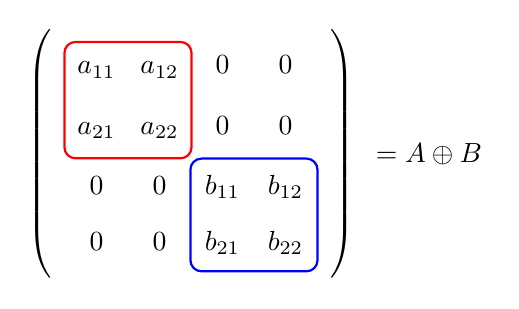
\begin{tikzpicture}
\matrix (m) [matrix of math nodes, left delimiter=(, right delimiter=), nodes={minimum width=8mm, minimum height=7mm}] {
a_{11} & a_{12} & 0 & 0 \\ a_{21} & a_{22} & 0 & 0 \\ 0 & 0 & b_{11} & b_{12} \\ 0 & 0 & b_{21} & b_{22} \\ };
\draw[red, thick, rounded corners] (m-1-1.north west) rectangle (m-2-2.south east);
\draw[blue, thick, rounded corners] (m-3-3.north west) rectangle (m-4-4.south east);
\node[right=5mm of m] {$= A \oplus B$};
\end{tikzpicture}
\end{document}
